\documentclass[journal]{IEEEtran}

\renewcommand\thesection{\arabic{section}} 
\renewcommand\thesubsectiondis{\thesection.\arabic{subsection}}
\renewcommand\thesubsubsectiondis{\thesubsectiondis.\alph{subsubsection}}
\renewcommand\theparagraphdis{\arabic{paragraph}.}

%\usepackage[retainorgcmds]{IEEEtrantools}
%\usepackage{bibentry}  
\usepackage{xcolor,soul,framed} %,caption

\colorlet{shadecolor}{yellow}
% \usepackage{color,soul}
\usepackage[pdftex]{graphicx}
\graphicspath{{../pdf/}{../jpeg/}}
\DeclareGraphicsExtensions{.pdf,.jpeg,.png}
\usepackage{authblk}
\usepackage[cmex10]{amsmath}
%Mathabx do not work on ScribTex => Removed
%\usepackage{mathabx}
\usepackage{array}
\usepackage{mdwmath}
\usepackage{mdwtab}
\usepackage{eqparbox}
\usepackage{url}
\hyphenation{op-tical net-works semi-conduc-tor}
\usepackage{graphicx}
\usepackage[T1]{fontenc}
\usepackage{dblfloatfix}     % To enable figures at the bottom of page




%\bstctlcite{IEEE:BSTcontrol}
%=== TITLE & AUTHORS ====================================================================
\begin{document}

\bstctlcite{IEEEexample:BSTcontrol}
    \title{
    	
\includegraphics[width=5in]{../imgs/madi_logo.png} 
    	\newline
    	\newline
     Representation Learning for Gait Analysis in Parkinson's Patients \\ 
     }

\author{Tim Löhr}
\author{Christoph Popp}
\affil{Department of Computer Science, University of Erlangen-Nürnberg}




% The paper headers
\markboth{Final Paper for the Machine Learning Timeseries Project at the Machine Learning and Data Analytics Lab at the FAU 
}{Roberg \MakeLowercase{\textit{et al.}}}


% ====================================================================
\maketitle
% === ABSTRACT 
\begin{abstract}
%\boldmath
This project aims to quantify how accurately Morbus Parkinson's can be classified by different types of deep learning architecture without preprocessing the original sensor data. For this purpose, four different architectures (LSTM, ResNet, a basic autoencoder and a ResNet autoencoder) were used to evaluate the accuracy. The data was collected from patients at the University Hospital of Erlangen. Different severity levels of Parkinson's were regarded as being deceased. In this regard, this project performed a binary classification task (healthy and deceased). It shows, that a ResNet autoencoder predicts Parkinson with 87\% accuracy and can be used as a decision support system for doctors. 
\end{abstract}

% === KEYWORDS 
\begin{IEEEkeywords}
Machine Learning Timeseries, Parkinson, Data Analysis, Gait Analysis, Neural Networks, FAU, Department of Computer Science
\end{IEEEkeywords}

\IEEEpeerreviewmaketitle

% === I. Project background and motivation
\section{Introduction}
\IEEEPARstart{H}{}ospitals in Germany are digitizing their workflows more and more every year \cite{cite2}. This offers great opportunities to make use of large amounts of collected medical data or being able to collect data in a novel way, for example with different kinds of sensors. Machine Learning and Deep Learning models can be efficiently and cheaply applied by supporting doctors to identify diseases.
Morbus Parkinson is the second most common neurodegenerative disease after Alzheimer with around 250.000 to 280.000 affected people in Germany alone \cite{cite1}. A common way to test if a patient is deceased with Parkinson's is the L-Dopa test. This drug can reduce the complaints of patients with only a high single dosage. On the contrary, the risk of possible side effects rises by the younger the patients are \cite{cite3}. For this reason, the highest priority in our classification task is to reduce the number of false-positives as much as possible, especially when taking age into consideration. 
The background of this project is, that we wanted to know how well we can predict Parkinson with sensor data that underwent no special preprocessing, only feature normalization.

The research question for this project can therefore be concluded as:
\\ 
\textit{Can Deep Learning be safely applied as decision support for doctors to identify Morbus Parkinson with normalized sensor data?}

% === II. Procedural Method==================================== 
\section{Methods}
For this dataset, the hospital in Erlangen measured 290 patients with three sensors on each foot. The sensors have been attached to the feet of the patients and they were told to walk 4 times 10 meters. In most cases, the time-series data reveals the turns after every 10 meters of the walk as can be seen in Figure \ref{fig:features}, where the time-series shows four distinct sections. 

\begin{figure}
\centering
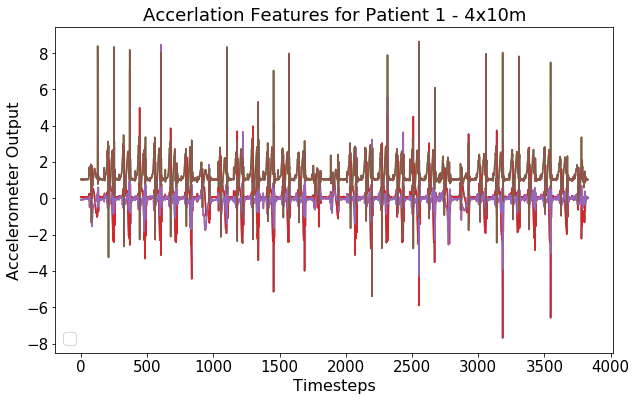
\includegraphics[width=1\linewidth]{../imgs/features}
\caption{Timeseries Plot of the acceleration features of patient 1}
\label{fig:features}
\end{figure}

It is split up into two-thirds of Parkinson deceased patients and one-third of healthy patients. Based on the \textit{UPDRS} (Unified Parkinson’s Disease Rating Scale), there exist seven levels of severity of Morbus Parkinson. For our experiments, we only took into consideration whether or not a patient has Parkinson's, not how severe the disease is. There is also the metric \textit{Hoehn Yahr}, which gives an indication of the severity. We regard patients as healthy if both the UPDRS and the Hoehn Year metric shows a 0. So even if patients have Parkinson's on the best or worst possible condition, we regard everything as sick. Therefore, we have a binary classification problem.

The mean age of the patients from this dataset is distributed normally around 60 years (Figure \ref{fig:age}). This is also the most common age for people to be affected by this disease \cite{cite3}. 

\begin{figure}
\centering
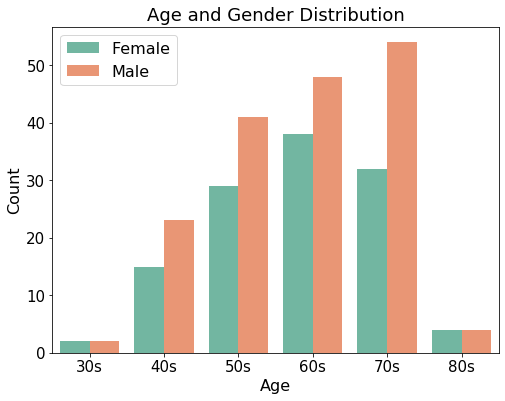
\includegraphics[width=1\linewidth]{../imgs/age}
\caption{Age and gender distribution of the 290 patients}
\label{fig:age}
\end{figure}

The measurement of the six sensor results in twelve features per patient, because every sensor has an x and y measurement. On some occasions, the left-foot and right-foot data needed to be aligned. Furthermore, one row in the dataset does not necessarily indicate one second. The length of each patient's data varies a lot by length. The shortest measurement has around 2000 rows, whereas the longest has 16000 (Figure \ref{fig:timeseries}) with a median value of 4000 rows.  

\begin{figure}
\centering
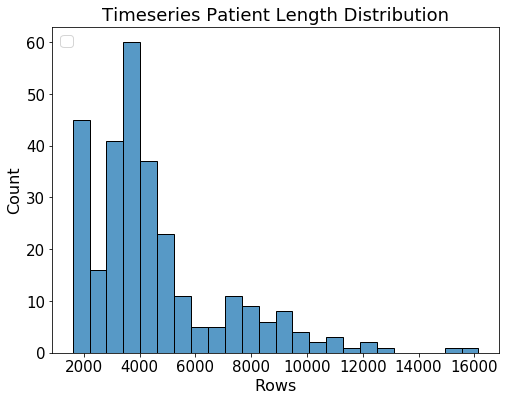
\includegraphics[width=1\linewidth]{../imgs/timeseries}
\caption{Distribution of the length of the timeseries data for the 290 patients}
\label{fig:timeseries}
\end{figure}

A recurrent neural network does not care about the input length. For the convolutional neural networks, we needed to make a fixed cut at a certain length and padded data that is shorter than the cut with zeros. We tested our binary classification task with four different Deep Learning approaches:

\begin{itemize}
\item Long Short Term Memory (LSTM)
\item ResNet (CNN)
\item Autoencoder Sampler
\item Autoencoder Reconstruction Error
\end{itemize}

The models needed to be prepared in very different manners. Architectures and hyperparameters were tested differently for each model. 

\subsection{LSTM}
The LSTM was the first attempted to model the binary classification task. Recurrent neural networks are often used for time-series tasks. The LSTM could be able to find patterns in the timeframes, that indicates if the person is deceased. Parkinson often leads to a trembling walking \cite{cite1}, so the LSTM possibly captures the trembling in the sensor data. We used a very basic architecture with:

\begin{itemize}
\item Input size: 12 (features)
\item Hidden size: 256
\item Number of Layers: 5
\end{itemize}

The hidden size and the number of layers were chosen as commonly used default values. Leaky ReLU's are additionally used and fully connected layers, which resolve in a scaler output which is used to compute the binary entropy loss for the binary classification. 

\subsection{ResNet}
The second approach for the classification task was to use a convolution architecture to find patterns in the data. A common architecture is the ResNet, which is usually used in image classification tasks. Besides the ResNet architecture, there are many different ones, which could be used like the Inception architecture or the classic AlexNet. All of those architectures are relatively old and because of that we also considered a newer architecture called EfficientNet. The main idea here is to let the network learn the size of the convolution operation instead of fixing it. Yet, after some runs this architecture did not seem to work for our problem, providing significantly worse results than the simple ResNet. This is the reason we concentrated on the improvement of the ResNet architecture. We ended up with the usage of four Resblocks consisting of two convolution layers, two batchnorm layers, two relu activation functions and one one-by-one convolution layer in the order: convolution, batchnorm, relu, convolution, batchnorm, relu, 1x1 convolution.\\Before the Resblocks one convolution layer was used with a relu activation function and a maxpooling layer. After the last Resblock one averagepooling layer was used and the flattened output was fed into three fully-connected layers with exponential linear unit (ELU) activation functions and a dropout chance of 20\%. To get the binary classification result, as the last layer another fully-connected layer was used together with a sigmoid activation function to map the output values to a range from 0 to 1. The last layers used an ELU activation function instead of a relu to minimize the vanishing gradient problem. All the other building blocks are used as in a classic ResNet. For training, the binary-cross-entropy loss was used, since this is the standard loss for binary classification problems. As an optimizer, Adam was the right choice with a learning rate of 8e-4, because other optimizers, like simple SGD, produced outputs that were always very close to each other.

\subsection{Autoencoder}
The classical autoencoder consists of two parts as shown in Figure \ref{fig:autoencoder}:
\begin{itemize}
\item Encoder
\item Decoder
\end{itemize}

\begin{figure}
\centering
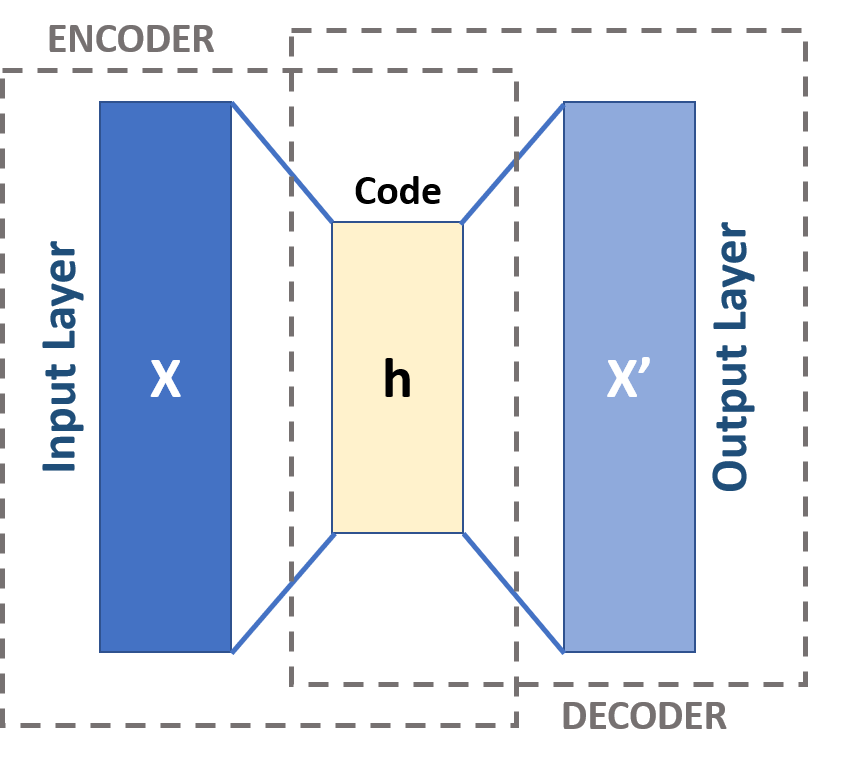
\includegraphics[width=1\linewidth]{../imgs/autoencoder}
\caption{Basic autoencoder architecture, Image from Wikipedia}
\label{fig:autoencoder}
\end{figure}

The encoders architecture can be freely designed as long as the input is downsampled to a bottleneck vector \textbf{h} like in Figure \ref{fig:autoencoder}. The bottleneck vector can be as small as a scaler value, but a higher dimension is also possible. For non-linear activation functions, the autoencoder behaves like a Principal Component Analysis (PCA).
The lower-dimensional representation of the data is upsampled again by the decoder. The MSE loss (Mean Squared Error) can be calculated by the difference of the original input and the downsampled and back upsampled input. Ideally, the networks learn how to reduce the dimensionality of the input data in the bottleneck layer and can reconstruct the original image from the downsampled version perfectly without a loss of information.
There exist multiple ways in which an autoencoder can be applied and designed. For our project, we implemented two possible ways of classifying the sensor data binary.

We also decided on a fixed-length time-series size of 8192 for both of our autoencoder networks. Due to the median length of data being around 4000 rows long, most data is padded at least a little bit with zeros at the end. Still, the networks have shown to increase their accuracy clearly by doubling the first attempted block size of 4096 to 8192. This makes intuitive sense because more data can be used to train the networks.

\subsubsection{Autoencoder Sampler}
The autoencoder sampler is trained both on the healthy and diseased patients. This enables the network to both classify and also sample new healthy and deceased data from the model. For this architecture, three networks have to be trained:

\begin{itemize}
\item Encoder
\item Decoder
\item Classification Network
\end{itemize}

The training data is sampled down by two fully connected layers into a 4D bottleneck layer. 

\begin{itemize}
\item Fully Connected Layer from 8192*12 into 128
\item ReLU activasion function
\item Fully Connected Layer from 128 to 4
\end{itemize}

The dimensionality reduction from 12 features into 4D is then used to simultaneously train a small classification network, consisting also of fully connected layers and ReLU activation functions. The networks try to make a binary decision based on the 4D dimensionality reduced data. The downsampled 4D data is then decoded back and upsampled into the original shape and the loss is computed by adding up both the decoder loss and the classification network's binary cross-entropy loss (BCE).

\subsubsection{Autoencoder Reconstruction Error}
The autoencoder sampler is trained only on the healthy patients' data. In this case, we would only be able to sample healthy patient's data, which has no benefit for sampling tasks. The main purpose of the network is therefore only the binary classification.

For this autoencoder, a deeper architecture has been chosen, because the sampling autoencoder appeared to be not complex enough with too few parameters. The classical ResNet from chapter 2.2 is used as the encoder architecture, and the reversed ResNet is used as the decoder to upsample the bottleneck vector back into its original input shape. This huge network has 47.1 million parameters to train on. Since the ResNet alone worked very well, it appeared that the ResNet architecture could work even better when applied to an autoencoder.

The reconstruction loss is ideally zero when training and predicting only healthy patients. The idea is to use the reconstruction loss after the training for making novel predictions on Parkinson's deceased patients. Since the network has not seen any Parkinson data yet, the reconstruction loss should be greater than zero and a threshold can be set to classify between healthy and Parkinson.
%
%==================================================
%
\section{Results} 
\subsection{LSTM}
After training the network for 100 epochs, the network predicted every patient as being Parkinson's deceased. Due to unbalancing factor is two-thirds of sick patients, the accuracy was 66\%. No matter with which learning rate or deeper architectures of the LSTM architecture, the network did not start learning how to classify properly. 

\subsection{ResNet}
As already mentioned in the ResNet subsection we focused on the ResNet, because it gave us the best output from all other architectures. To get a feeling for what a good output is we have to notice that our dataset was imbalanced, containing 2/3 of Parkinson's and only 1/3 healthy data. Because of that imbalance, an accuracy of around 66\% can already be achieved by classifying each input as Parkinson's disease. First, let us have a look at the training loss and training accuracy of the model.\\

The reconstruction loss is ideally zero when training and predicting only healthy patients. The idea is to use the reconstruction loss after the training for making novel predictions on Parkinson's deceased patients. Since the network has not seen any Parkinson data yet, the reconstruction loss should be greater than zero and a threshold can be set to classify between healthy and Parkinson.
\begin{figure}
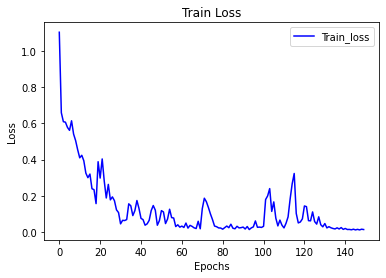
\includegraphics[width=1\columnwidth]{../imgs/train_loss_resnet.png}
\caption{Training loss of the binary cross entropy function}
\end{figure}
\begin{figure}
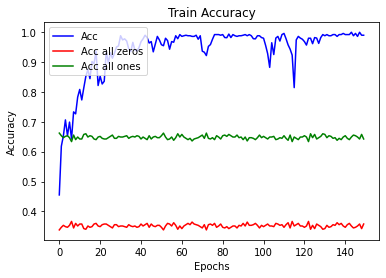
\includegraphics[width=1\columnwidth]{../imgs/train_accuracy_resnet.png}
\caption{Training accuracy of the ResNet}
\end{figure}
It can be seen that the loss curve goes down as expected and the accuracy always gets closer to 100\%. This is good because that way we can be sure that our model is learning something and is not just predicting random things. The negative part is that once the training accuracy gets close to 100\% it is very likely that our model is overfitting to the training data, which results in a worse result in the validation data. Next comes the validation loss.\\
\begin{figure}
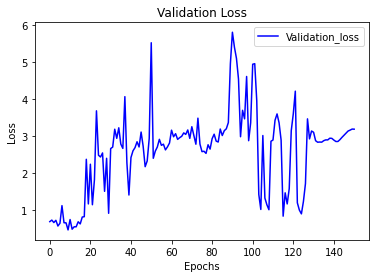
\includegraphics[width=1\columnwidth]{../imgs/validation_loss_resnet.png}
\caption{Validation loss of the binary cross entropy function}
\end{figure}
\begin{figure}
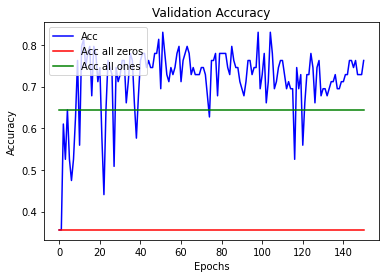
\includegraphics[width=1\columnwidth]{../imgs/validation_accuracy_resnet.png}
\caption{Validation accuracy of the ResNet}
\end{figure}

Here it can be seen that the curves are not as smooth as the ones for the training. The accuracy here is varying around 75\% with a small downward trend for higher epoch numbers. This downward trend can be caused by the overfitting of the network. Also, it is not clear what role the padding with zeros in the data plays. This could have been also a reason why the accuracy is not increasing more.\\All in all the accuracy is way above the threshold of 66\% with peaks of 82\% or even 88\% depending on the initialization, which shows that the network is learning a representation of the data and not just the classification of every input to one or zero.

\subsection{Autoencoder Sampler}
The sampling autoencoder was the first approach for the autoencoder architecture. It appeared that even after 150 epochs of training, the simple fully connected architecture was not capable of training a model that can simultaneously train on healthy and sick data. The reconstruction loss for both the healthy and sick patient's data was completely arbitrary and no proper classification could be done.

\subsection{Autoencoder Reconstruction Error}
Since the classical ResNet worked well, an autoencoder with the same kind of architecture could work as well. When training only on the same label (healthy), the network is expected to heavily overfit the healthy patient's data. After 200 epochs of training the loss converged to a fixed 0.23 value (Figure \ref{fig:ac_loss}).

\begin{figure}
\centering
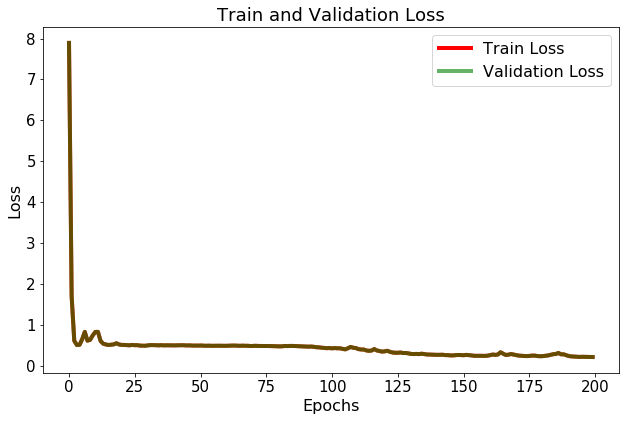
\includegraphics[width=1\linewidth]{../imgs/ac_loss}
\caption{Train and Validation loss of the reconstruction loss autoencoder}
\label{fig:ac_loss}
\end{figure}

A test dataset with 13 healthy and 10 deceased patients was used to make predictions based on the reconstruction loss. It showed, that the best accuracy of 87\% was achieved with a threshold value of 0.2, as shown in Figure \ref{fig:ac_accuracy}.

\begin{figure}
\centering
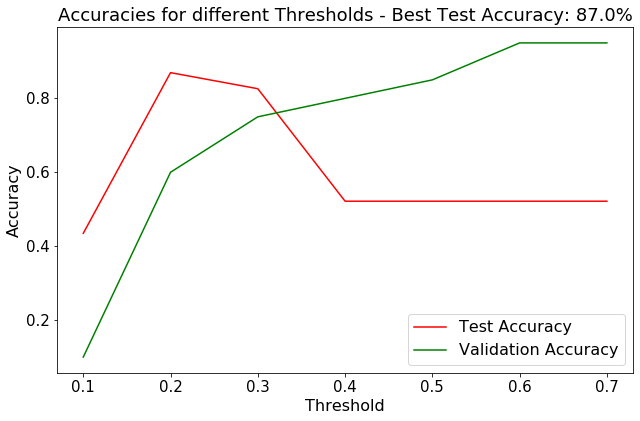
\includegraphics[width=1\linewidth]{../imgs/ac_acc}
\caption{Train and Validation accuracy of the reconstruction loss autoencoder}
\label{fig:ac_accuracy}
\end{figure}

When looking at Figure \ref{fig:ac_accuracy}, the validation accuracy quickly rises to 100\%, because the validation dataset consists only out of healthy like the training dataset. Therefore, the accuracy must rise to 100\% when further enhancing the threshold. The test accuracy has its peak at 0.2, but the greater the threshold is increased, the more false-positive are reduced. So ideally, when wanting a 95\% certainty for not having any false positives, the threshold must be set so high until this constraint is satisfied. This is the advantage of the autoencoder with classification on the reconstruction loss over the classical ResNet classification. 

\begin{figure}
\centering
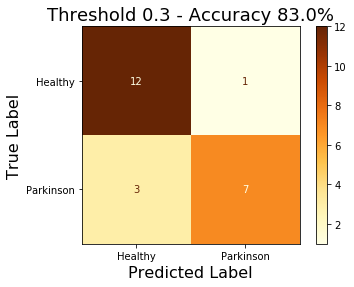
\includegraphics[width=1\linewidth]{../imgs/confusion_matrix}
\caption{Confusion Matrix for the treshold 0.2 with the accuracy of 87\%}
\label{fig:ac_cm}
\end{figure}

The confusion matrix in Figure \ref{fig:ac_cm} reveals exactly this. By further increasing the threshold, the false-positives (lower left) will decrease, whereas the false-negatives (upper right) will increase. People left undetected with Parkinson's increase, but no patient is harmed due to medication for a false treatment.
%
% === II. 4	Data description with visualization==========================
%
\section{Discussion}
The experiments showed, that a convolution-based architecture like the ResNet performs better than recurrent based neural network architectures. The ResNet itself was developed in 2012, so there exist much more modern architectures with more parameters. The results show that CNN based architectures perform reasonably well, but it is not clear what the models have exactly been learning. The big difference in rows for each patient led to many problems for performing the training. Still, there is no clear indication that more data means a patient has Parkinson's, which would be a reasonable assumption since Parkinson's deceased people walk generally worse than healthy people and therefore need more time and rows. Since this was assumption was false, it appears the network learned the difference in some sense. Nevertheless is the autoencoder approach more useful than the basic ResNet architecture, because it enables us to adjust the threshold and accordingly uses this to adjust for a minimum false-positive or false-negative ratio. 
After considering all evaluation steps, can Deep Learning be safely applied as decision support for doctors to identify Morbus Parkinson with normalized sensor data?

\textbf{Pros}
\begin{itemize}
\item Cheap and easy decision support
\item Arbitrary threshold enables adjustment of the false-positive rate
\item Age can be taken separately into consideration after the prediction
\item The accuracy of 87\% indicates some level of certainty
\item Sampling of healthy patient data is possible
\end{itemize}

\textbf{Cons}
\begin{itemize}
\item The prediction allows no medical evidence at all
\item It is unclear what the network exactly learned
\item More data is required
\end{itemize}

The autoencoder with reconstruction loss can be used as cheap decision support for doctors in the future, also for various other diseases, this project can be used as a template, because most sensor data does not vary that much from each other.


\section{Conclusion}
The conclusion of this project leads to three finals questions:

\textit{Can we classify without any special kind of preprocessing?}
The results have shown, that the Resnet and the autoencoder with reconstruction loss have a performance of 87\% accuracy. Without any further bayesian optimization or a deeper network, this indicates that the networks could even improve further. The answer to this question is a clear yes. 

\textit{Which network architecture performs the best?}
After the experiments, it showed that recurrent models could not capture the complexity of the task at all. CNN based architecture worked the best for this project.

\textit{Does the accuracy and prediction provides evidence that the network clearly understands the difference between Parkinson deceased and healthy patients?}
No clinical evidence at all. There is a possibility, that the network only learned the padding at the end of each fixed batch block of length 8192, even though the was no clear evidence that larger time-series data indicate Parkinson's disease.

\section{Future Work}
More adjustment can be made for future experiments:

\begin{itemize}
\item Using a more modern network architecture for the autoencoder like the Efficient Net
\item Use bayesian optimization for the batch size and learning rate
\item Train more epochs
\end{itemize}


% if have a single appendix:
%\appendix[Proof of the Zonklar Equations]
% or
%\appendix  % for no appendix heading
% do not use \section anymore after \appendix, only \section*
% is possibly needed

% use appendices with more than one appendix
% then use \section to start each appendix
% you must declare a \section before using any
% \subsection or using \label (\appendices by itself
% starts a section numbered zero.)
%

% ============================================
%\appendices
%\section{Proof of the First Zonklar Equation}
%Appendix one text goes here %\cite{Roberg2010}.

% you can choose not to have a title for an appendix
% if you want by leaving the argument blank
%\section{}
%Appendix two text goes here.


% use section* for acknowledgement
%\section*{Acknowledgment}


%The authors would like to thank D. Root for the loan of the SWAP. The SWAP that can ONLY be usefull in Boulder...


% Can use something like this to put references on a page
% by themselves when using endfloat and the captionsoff option.
\ifCLASSOPTIONcaptionsoff
  \newpage
\fi



% trigger a \newpage just before the given reference
% number - used to balance the columns on the last page
% adjust value as needed - may need to be readjusted if
% the document is modified later
%\IEEEtriggeratref{8}
% The "triggered" command can be changed if desired:
%\IEEEtriggercmd{\enlargethispage{-5in}}

% ====== REFERENCE SECTION

%\begin{thebibliography}{1}

% IEEEabrv,

\bibliographystyle{IEEEtran}
\bibliography{IEEEabrv,Bibliography}
%\end{thebibliography}
% biography section
% 
% If you have an EPS/PDF photo (graphicx package needed) extra braces are
% needed around the contents of the optional argument to biography to prevent
% the LaTeX parser from getting confused when it sees the complicated
% \includegraphics command within an optional argument. (You could create
% your own custom macro containing the \includegraphics command to make things
% simpler here.)
%\begin{biography}[{\includegraphics[width=1in,height=1.25in,clip,keepaspectratio]{mshell}}]{Michael Shell}
% or if you just want to reserve a space for a photo:

% ==== SWITCH OFF the BIO for submission
% ==== SWITCH OFF the BIO for submission


%% if you will not have a photo at all:
%\begin{IEEEbiographynophoto}{Ignacio Ramos}
%(S'12) received the B.S. degree in electrical engineering from the University of Illinois at Chicago in 2009, and is currently working toward the Ph.D. degree at the University of Colorado at Boulder. From 2009 to 2011, he was with the Power and Electronic Systems Department at Raytheon IDS, Sudbury, MA. His research interests include high-efficiency microwave power amplifiers, microwave DC/DC converters, radar systems, and wireless power transmission.
%\end{IEEEbiographynophoto}

%% insert where needed to balance the two columns on the last page with
%% biographies
%%\newpage

%\begin{IEEEbiographynophoto}{Jane Doe}
%Biography text here.
%\end{IEEEbiographynophoto}
% ==== SWITCH OFF the BIO for submission
% ==== SWITCH OFF the BIO for submission



% You can push biographies down or up by placing
% a \vfill before or after them. The appropriate
% use of \vfill depends on what kind of text is
% on the last page and whether or not the columns
% are being equalized.

\vfill

% Can be used to pull up biographies so that the bottom of the last one
% is flush with the other column.
%\enlargethispage{-5in}



% that's all folks
\end{document}